\subsection{Copy Optimized Blocks}
The \ttt{copyopt} kernel presented in \secref{opt} performs well for small
matrices, but performs poorly for large matrices. More specifically, when the
matrix does not fit in L3 cache, the naive matrix multiplication algorithm
exhibits poor spatial locality which significantly limits performance.

To adopt the benefits of copy optimization without the disadvantage of poor
cache locality, we created the \ttt{big\_blocked} kernel: a kernel that uses
copy optimization and a blocked data access pattern. Concretely, the
\ttt{big\_blocked} kernel performs a blocked matrix multiplication in which a
block $A_{ik}$ of $A$ is multiplied by a block $B_{kj}$ of $B$ to produce a
block $C_{ij}$ of $C$. Before each block multiplication, $A_{ik}$ is copied
into a buffer in row-major order.

We performed a parametric sweep on the block size of the \ttt{big\_blocked}
kernel to decide on an optimal block size. The results of the sweep can be
found in \figref{block-sweep}. A block size of \todo{???} was selected.

\begin{figure}[h]
  \centering
  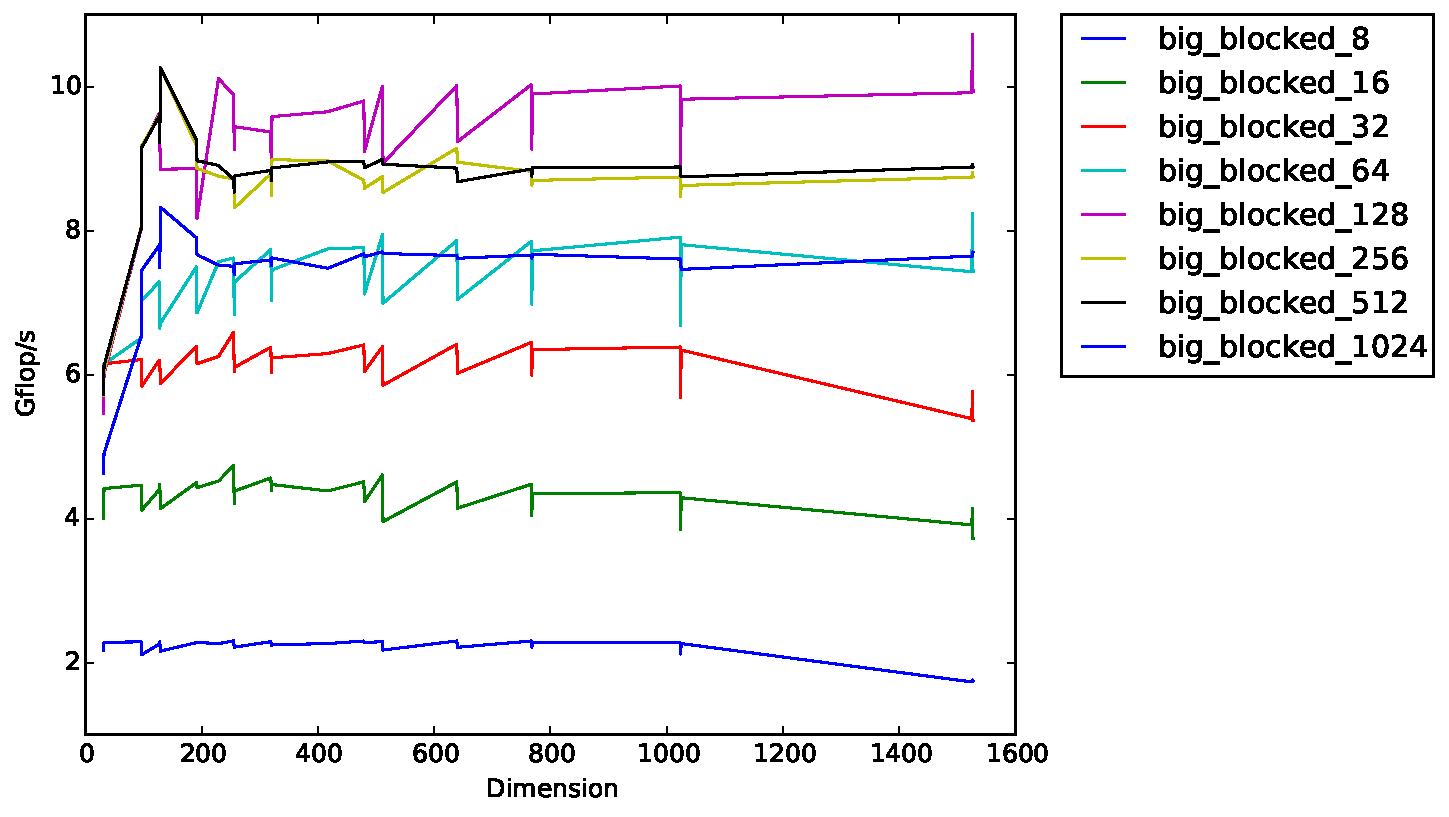
\includegraphics[width=\textwidth]{img/timing_big_block_sweep.pdf}
  \caption{Parametric sweep of block size for the \ttt{big\_blocked} kernel.}
  \label{fig:block-sweep}
\end{figure}
